\chapter{Design of the language}
In the Design chapter I am going to talk about how the language and the plugin have been designed and how they work.

\section{Introduction}
The idea was to think of a language that could implement all the possible actions which a security tester would be wanting to do on a multipart webapp test. One of the objective was to think of a language that could define tests that could be defined once, but tested over multiple websites. For example, a series of tests to verify the well-known vulnerabilities of a particular protocol could be defined and then used on any type of website.
I had to decide how to write and define the actual tests, i thought i could define a proper language with a dedicated parser, but it was not worth the effort, as there are already some well-tested alternatives available. I found a great alternative: i used JSON as a base over which write the tests. It is a convinient way of defining gerarchical sturctures like tests could be.
The idea behind this language is that a specific message can be intercepted and checked or edited in some way, to do this we define various types
The gerarchical structure and the details of the language will be discussed in the next charapter.

\section{Test example: PKCE Downgrade}
I want to introduce the language with an example. Due to its complexity, having a real example before the explanation of all its components could be helpful to understand their use.
The implemented test has as objective to test an OAuth vulnerability where removing the parameter "code\_challenge" from the url of an authorization request message will be downgrading the authentication proces in a way that PKCE will not be used if the service is vulnerable.


\begin{lstlisting}[language=json]
{
    "test suite": {
        "name": "OAuth Active tests",
        "description": "A series of tests to test OAuth's well-known vulnerabilities"
    },
    "tests": [    
        {
            "test": {
                "name": "PKCE Downgrade",
                "description": "Tries to remove code_challenge parameter",
                "type": "active",
                "sessions": [
                    "s1"
                ],
                "operations": [
                    {
                        "session": "s1",
                        "action": "start"
                    },
                    {
                        "action": "intercept",
                        "from session": "s1",
                        "then": "forward",
                        "message type": "authorization request",
                        "preconditions": [
                            {
                                "in": "url",
                                "check param": "code_challenge",
                                "is present": true
                            }
                        ],
                        "message operations": [
                            {
                                "from": "url",
                                "remove parameter": "code_challenge"
                            }
                        ]
                    }
                ],
                "result": "incorrect flow s1"
            }
    
        }
    ]
}
\end{lstlisting}

The first Operation defined in this test at line 17 is an operation that is used to start the session (and the browser). The automated browser will execute a series of actions defined by the user in a session track. The actions in this case will do a complete login in a website that uses OAuth as SSO login option. During the execution of the actions, language's Operations will be executed. At line 21 there is an Operation used to intercept an "authorization request" message, that is defined in an apoosite file where all Message Types are defined. Once an authorization request message is intercepted, the preconditions at line 32 are executed, checking that the parameter we want to test the vulnerability is used. This is done because the parameter "code\_challenge" is not an optional parameter for the OAuth protocol, so, if it is not present, i want the test to result "not applicable" instead of failed or passed.
The next part of the example is the Message Operation at line 35, where I tell to remove from the intercepted message's url the "code\_challenge" parameter.
The last part of the test is the definition of the result, the result is part of the evaluation of a test, in this case it is set to "incorrect flow s1", this means that I want the test to be considered passed if the execution of the session s1 is incorrect that is, if the execution of the session s1 encounters an error or an unexpected page.


\section{Language structure}
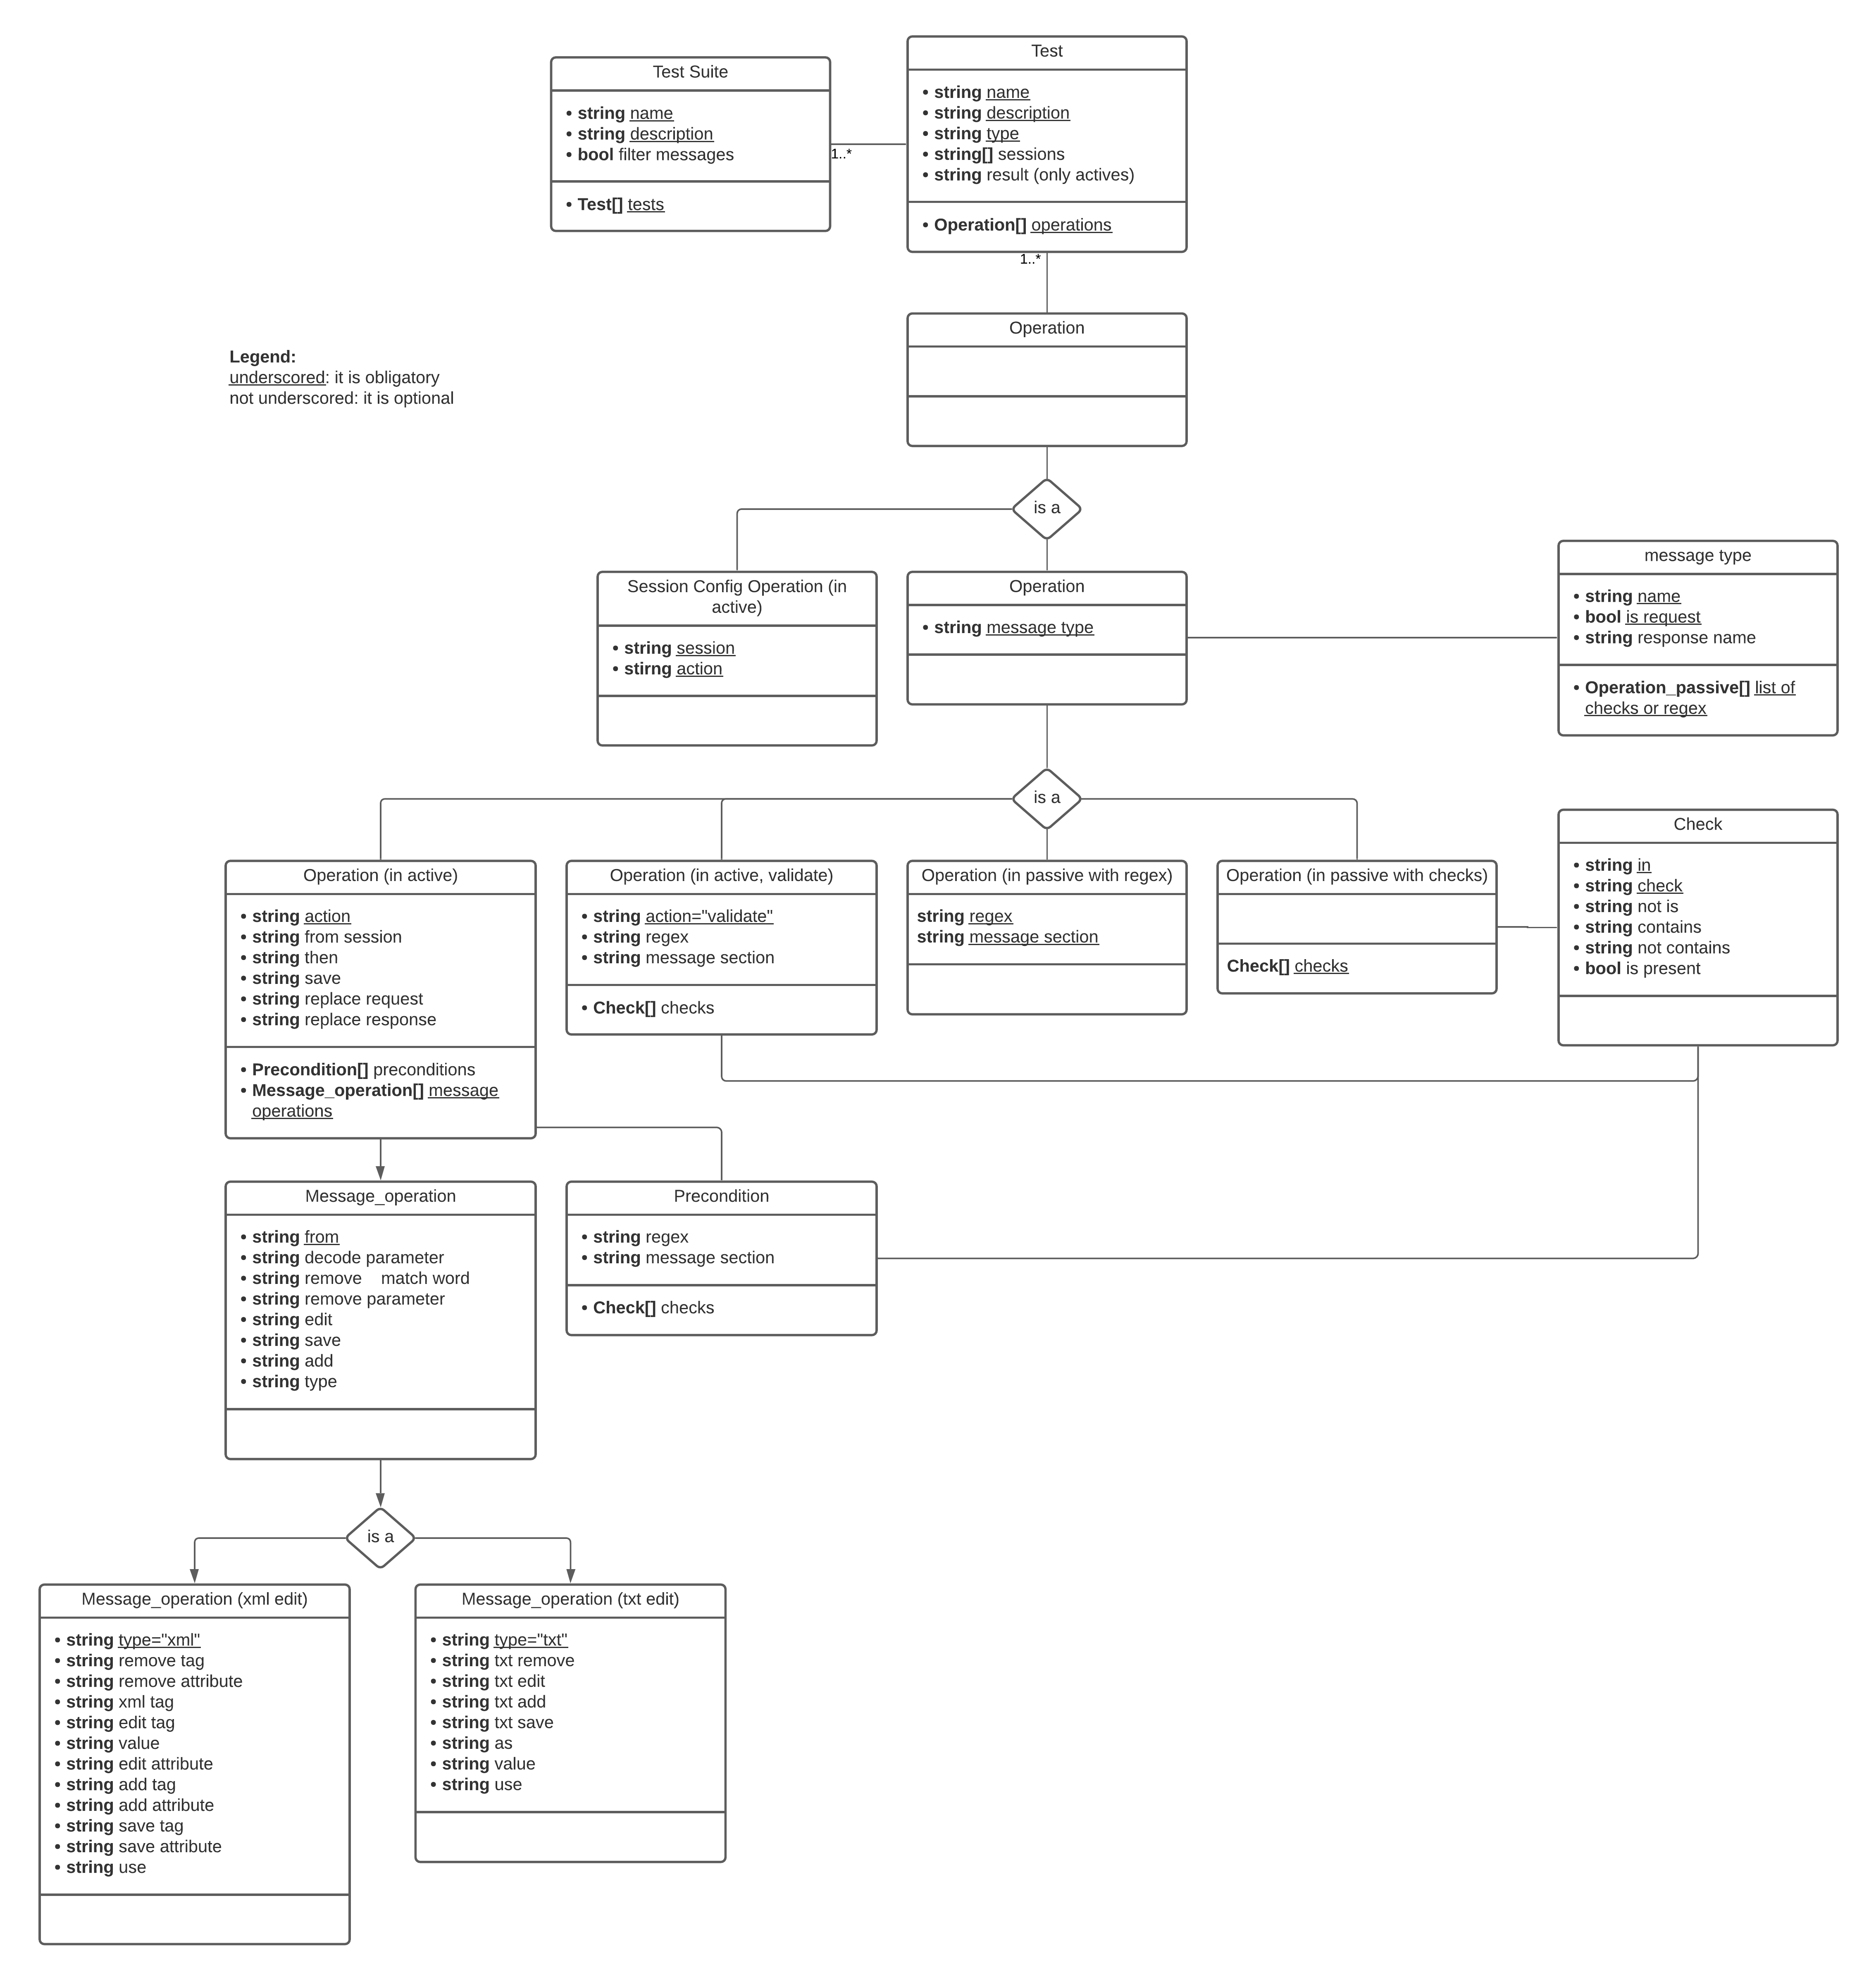
\includegraphics[width=\textwidth]{language_structure.png}

\subsection{Test suite}
The test suite is the main component which contains all the other one, it is composed by:
\begin{itemize}
    \item Test suite name, the name of the test suite
    \item Test suite description, the description of the test suite
    \item Tests, which is a list containing the tests to be executed
\end{itemize}

\subsection{Test}
The Test object is the one that actually defines a test. As said earlier, a test is contained in a Test Suite, and has various items:
\begin{itemize}
    \item name
    \item description
    \item type, it can be "active" or "passive"
    \item sessions, which is a list of the sessions which are needed in this test
    \item result, (only for actives) it defines the conditions over which the test is considered passed or not.
    \item operations, a list of operation objects which will be executed in the Test object
\end{itemize}

it can be defined either as an active or a passive test, depending on the type of actions it has to do on the intercepted messages. If a test doesn't need to manipulate the flow or the content of the messages, then it is considered passive, otherwise it is considered active.
The list of Operations contained in a Test is executed iteratively one after the other.

\subsection{Operation}
The operation object is the thing that define what a test actually does. As shown in the image above, an operation could be either a standard operation or a session config operation, the latter is used to manage the sessions for the active tests (i.e. start, stop, pause). Depending on the type of test which an Operation is defined into, the standard Operation can be active or passive.
In both cases, an operation has to contain the \textbf{message type} which defines the type of message to be intercepted in that particular operation (more info in the dedicated paragraph).
\\A \textbf{passive} operation has as objective to verify the presence (or absence) of some text or parameters in the intercepted message, it should contain one of the following options:
\begin{itemize}
    \item A list of Check objects, which are then executed to check the presence of some text or parameter
    \item A regex inspection, which executes a inspection considering the intercepted message as plain text and executing a regex over it, if the regex has a match, the operation is considered passed, otherwise failed. Note that when a regex is used, it has to be specified also the message section over which to be executed (boy,head, url)
\end{itemize}

If the Test where the operations are defined is an \textbf{active} test, so if the intercepted messages need to be manipulated in some way, an active Operation has to be defined. It is composed by:
\begin{itemize}
    \item action, the action it has to do (intercept, validate)
    \item from session, from which session to expect the message to be intercepted
    \item then, the action to to after the receiving and manipulation of the message (forward or drop)
    \item replace request (or response), specify a previously saved message in order to replace it to the intercepted one
    \item preconditions, a list of Precondition objects
    \item message operations, a list of Message Operation objects, which will do the actual manipulation of the intercepted message
\end{itemize}

If the action is set to "\textbf{validate}" the operation becomes like a passive operation, because its objective is just to verify that some messages are as expected. It will contain or a regex or a list of checks to be done.

\subsection{Message Operation}
The message operation is the Object that actually does the manipulations on the intercepted messages. It is composed by:
\begin{itemize}
    \item from, the message section to work on
    \item decode parameter (optional) it indicates which parameter or string to be decoded before processed
    \item encodings (optional) the list of encodings to be applied to the parameter or text to be decoded. The supported encodings are base64, deflate, url
    \item remove match word (optional), remove text from te specified section in the matched message, it uses a regex
    \item edit, edit the matched text
    \item save, (optional) used to save an entire message in a variable in a way it can be used in future operations
    \item add, (optional) add some text after the matched text
    \item type (optional) specify the type of edit you want to do over a decoded parameter
\end{itemize}

In a message operation there is the possibility to specify a parameter or some text to be decoded before manipulation, to do that specify with "decode parameter" the parameter to be decoded and with "encodings" the encodings necessary to decode the parameter. The parameter (or text) decoded, at the end of the Message operation will be encoded again automatically.
The decoded parameter can be manipulated by means of the "\textbf{type}" tag, there is the possibility to intepreter the decoded parameter as plain text, and to edit it using some actions:
\begin{itemize}
    \item txt remove
    \item txt edit
    \item txt add
    \item txt save
\end{itemize}
All the previous tags accept a regex, and whatever that regex matches will be edited or added or saved.

Another possibility is to interpeter the decoded text as xml, assigning the type tag "xml".
This way we have various possible operations to be done on the xml:
\begin{itemize}
    \item remove tag
    \item remove attribute
    \item edit tag
    \item edit attribute
    \item add tag
    \item add attribute 
    \item save tag
    \item save attribute
\end{itemize}

\subsection{Message type definition}
The message type definition is needed in order to define some types of message that will be later used in the language to intercept them.
The message type definition is not actually part of the language, but it is stored in a file in the burp folder. Anyway, the definition of the type of messages uses the same Objects as the language.
A message type object is defined using these tags:
\begin{itemize}
    \item name, the name that will be used in the language to reffer to this message type
    \item is request, se to true if the searched message is a request, false otherwise
    \item response name, the name that will be used in the language to reffer to the response of the searched message
    \item checks, a list of Check objects used to identify the message. If evaluated to true, the message is considered found
\end{itemize}
This is an example that defines the saml request and the saml response messages

\begin{lstlisting}[language=json]
{
    "message_types": [
        {
            "name": "saml request",
            "is request": true,
            "checks": [
                {
                    "in": "url",
                    "check param": "SAMLRequest",
                    "is present": true
                }
            ]
        },
        {
            "name": "saml response",
            "is request": true,
            "checks": [
                {
                    "in": "body",
                    "check param": "SAMLResponse",
                    "is present": true
                }
            ]
        }
    ]
}
\end{lstlisting}
So, if "saml request" is used in an Operation, the message having the parameter SAMLRequest in his url will be intercepted an processed by the Operation.


\section{The oracle}
The ensemble of all parts of the language that decide the result of the tests is called Oracle,
the oracle decides whether a test should be considered passed or failed. I decided to build the oracle in a way that can be almost fully customized by the user. There are various components that belong to the oracle. If we take the example from above, we can see that the test has a tag "result" which value is "incorrect flow s1", this means that the oracle will evaluate the test as passed if and only if the execution of the session track of the session s1 will be incorrect, this means that if the browser will encounter some type of page which was not meant to encounter, the test will be considered passed. With "was not meant to encounter" i mean that the actions in the session track cannot be done, because the objects to be pressed in the page are not present.
With this check i also added the possibility to do preconditions on the tests, they are useful to check if a given test is applicable or not. For example, at line 25 in the example above, I want to consider the test "not applicable" if i can't find the parameter code\_challenge in the authorization request message. This means that is not possible to apply the given test if the preconditions are not satisfied.


\section{Sessions}
A session is defined by a session track, which is a series of commands that the browser will execute automatically during execution of the Tests. There is the possibility of defining and using more than one session, in a way that (i.e.) reply tests can be executed.
As said in the previous sections, a "from session" tag can be specified in the Operation, this will tell in which of the available session search the desired message. To define the session track I have used and extended the idea used in the Micro Id Gym tool \cite{claudio_grisenti}\cite{stefano_faccini}, adding some options like "wait" and "clear cookies" functionalities.
The syntax of the session track is based on the plain text export of Katalon Recorder\cite{katalon_recorder_syntax}.
An example of a session track:

\begin{lstlisting}[]
    open | https://www.google.com/ |
    click | id=L2AGLb |
    click | link=Accedi |
    click | id=identifierId |
    type | id=identifierId | matteo.bitussi@studenti.unitn.it
    click | id=identifierNext |
    click | id=clid |
    type | id=clid | matteo.bitussi@unitn.it
    click | id=inputPassword |
    type | id=inputPassword | password
    click | id=btnAccedi |
    click | link=Gmail |
\end{lstlisting}

This session track will do the login on the Unitn website using some credentials and password. The actions supported are:
\begin{itemize}
    \item open $|$ url $|$, to open an url
    \item click $|$ id=, link=, xpath= $|$, to click on a http object with the given id, link or xpath
    \item type $|$ id= $|$ text, to write on a given http element the given text
    \item wait $|$ milliseconds, to make the execution of the session wait for a given time 
    \item clear cookies $|$, to make the browser of the session clear all of the cookies in it
\end{itemize}



